% Options for packages loaded elsewhere
\PassOptionsToPackage{unicode}{hyperref}
\PassOptionsToPackage{hyphens}{url}
%
\documentclass[
]{article}
\usepackage{lmodern}
\usepackage{amssymb,amsmath}
\usepackage{ifxetex,ifluatex}
\ifnum 0\ifxetex 1\fi\ifluatex 1\fi=0 % if pdftex
  \usepackage[T1]{fontenc}
  \usepackage[utf8]{inputenc}
  \usepackage{textcomp} % provide euro and other symbols
\else % if luatex or xetex
  \usepackage{unicode-math}
  \defaultfontfeatures{Scale=MatchLowercase}
  \defaultfontfeatures[\rmfamily]{Ligatures=TeX,Scale=1}
\fi
% Use upquote if available, for straight quotes in verbatim environments
\IfFileExists{upquote.sty}{\usepackage{upquote}}{}
\IfFileExists{microtype.sty}{% use microtype if available
  \usepackage[]{microtype}
  \UseMicrotypeSet[protrusion]{basicmath} % disable protrusion for tt fonts
}{}
\makeatletter
\@ifundefined{KOMAClassName}{% if non-KOMA class
  \IfFileExists{parskip.sty}{%
    \usepackage{parskip}
  }{% else
    \setlength{\parindent}{0pt}
    \setlength{\parskip}{6pt plus 2pt minus 1pt}}
}{% if KOMA class
  \KOMAoptions{parskip=half}}
\makeatother
\usepackage{xcolor}
\IfFileExists{xurl.sty}{\usepackage{xurl}}{} % add URL line breaks if available
\IfFileExists{bookmark.sty}{\usepackage{bookmark}}{\usepackage{hyperref}}
\hypersetup{
  hidelinks,
  pdfcreator={LaTeX via pandoc}}
\urlstyle{same} % disable monospaced font for URLs
\usepackage{graphicx}
\makeatletter
\def\maxwidth{\ifdim\Gin@nat@width>\linewidth\linewidth\else\Gin@nat@width\fi}
\def\maxheight{\ifdim\Gin@nat@height>\textheight\textheight\else\Gin@nat@height\fi}
\makeatother
% Scale images if necessary, so that they will not overflow the page
% margins by default, and it is still possible to overwrite the defaults
% using explicit options in \includegraphics[width, height, ...]{}
\setkeys{Gin}{width=\maxwidth,height=\maxheight,keepaspectratio}
% Set default figure placement to htbp
\makeatletter
\def\fps@figure{htbp}
\makeatother
\setlength{\emergencystretch}{3em} % prevent overfull lines
\providecommand{\tightlist}{%
  \setlength{\itemsep}{0pt}\setlength{\parskip}{0pt}}
\setcounter{secnumdepth}{-\maxdimen} % remove section numbering

\author{}
\date{}

\begin{document}

\hypertarget{ux6a21ux578bux7684ux5efaux7acbux4e0eux6c42ux89e3}{%
\section{模型的建立与求解}\label{ux6a21ux578bux7684ux5efaux7acbux4e0eux6c42ux89e3}}

\hypertarget{ux95eeux9898ux4e00ux5e73ux884cux5e73ux9762ux8584ux819cux53ccux5149ux675fux5e72ux6d89ux7684ux5916ux5ef6ux5c42ux539aux5ea6ux6a21ux578b}{%
\subsection{问题一:平行平面薄膜双光束干涉的外延层厚度模型}\label{ux95eeux9898ux4e00ux5e73ux884cux5e73ux9762ux8584ux819cux53ccux5149ux675fux5e72ux6d89ux7684ux5916ux5ef6ux5c42ux539aux5ea6ux6a21ux578b}}

\hypertarget{ux5149ux7684ux632fux52a8ux51fdux6570}{%
\subsubsection{光的振动函数}\label{ux5149ux7684ux632fux52a8ux51fdux6570}}

时间变化的规律可以通过正弦函数和余弦函数来表述,其数学表达式为:

\[\overrightarrow{x}(t) = Acos(\text{ωt} + \varphi)\]

  \(\overrightarrow{x}(t)\):表示振动质点相对于其平衡位置的偏移量,用于描述质点在时刻 t 的位置。

  \(A\) :光矢量的大小表示振动质点偏离其平衡位置的最大距离,以米为单位,反映了振动的强度。

  \(\omega\) :角频率用于表征振动的速率,其单位为弧度/秒。它与频率 \(\nu\) 周期 \(T\) 的关系为 \(\omega = 2\text{πν} = \frac{2\pi}{T}\)。

  \(\varphi\) :初相位是指在t=0时刻的相位,单位为弧度,用于确定振动的初始条件。

\hypertarget{ux5149ux7684ux632fux52a8ux63cfux8ff0ux65cbux8f6cux77e2ux91cfux6cd5}{%
\subsubsection{光的振动描述------旋转矢量法}\label{ux5149ux7684ux632fux52a8ux63cfux8ff0ux65cbux8f6cux77e2ux91cfux6cd5}}

如图1所示,采用旋转矢量法表示,一矢量绕原点O以角速度ω逆时针匀速旋转,其瞬时在x轴上的投影即为光振动的简谐运动方程。

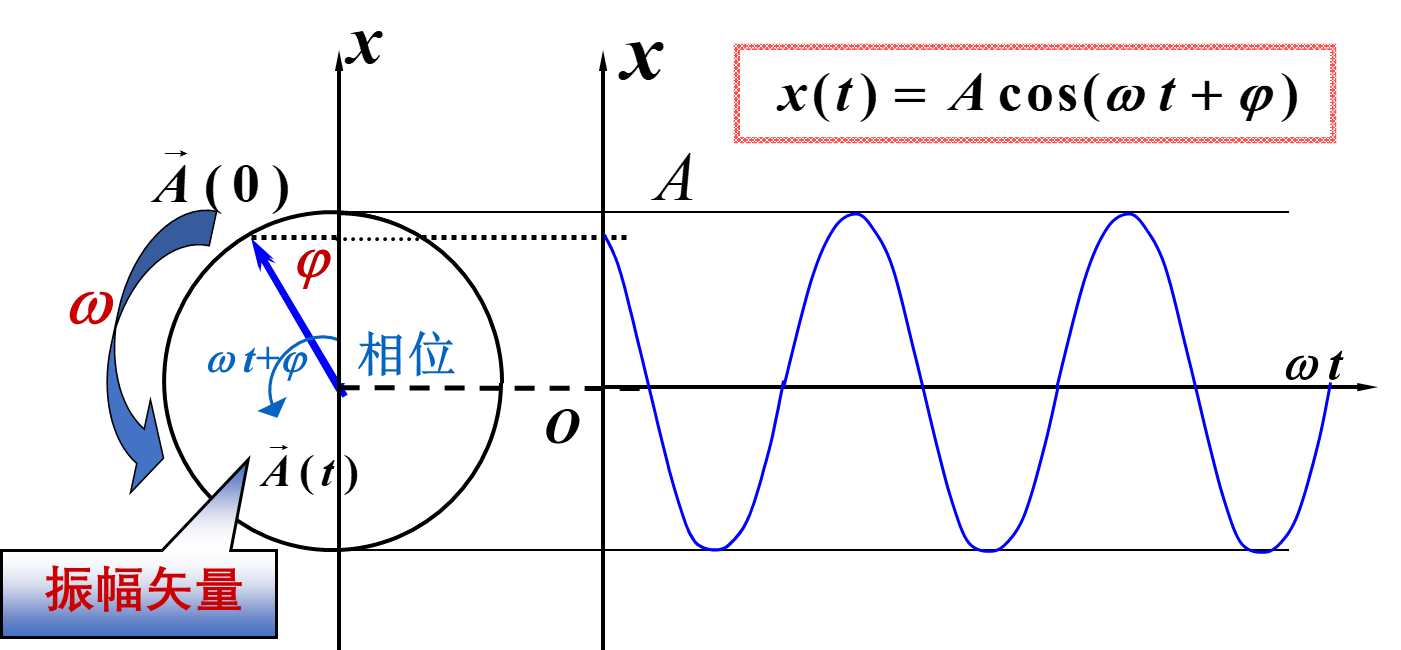
\includegraphics[width=4.81111in,height=2.23194in]{./media/media/image1.png}

图1 旋转矢量法表示光的振动方程

如图1所示,该图通过旋转矢量法(亦称相量法)阐述了简谐振动的两种等效表示。左侧为几何表示:一振幅为A的矢量绕原点O以角频率ω逆时针匀速旋转,其瞬时相位为ϕ=ωt。该矢量在纵轴(x轴)上的投影,即代表了振动系统在该时刻的瞬时位移x右侧为对应的时域表示,描述了上述投影随时间t的变化关系。如图所示,旋转矢量的运动精确地映射为一条以时间t为横轴、位移x为纵轴的正弦(或余弦)曲线,其数学表达为)x(t)=Acos(ωt+\(\varphi\)),与投影计算的结果完全一致。

旋转矢量法作为连接匀速圆周运动与一维简谐振动的桥梁,为理解振动参量提供了直观的几何图像:振幅A映射为旋转半径,决定了振动的强度;角频率~ω映射为旋转角速度,决定了振动的快慢;初相位ϕ0\hspace{0pt}映射为初始角位置,决定了振动的初始状态。这些几何关系清晰地解释了其时域波形x(t)=Acos(ωt+ϕ0)的特征。

\hypertarget{ux540cux65b9ux5411ux540cux9891ux7387ux7684ux5149ux7684ux5408ux6210}{%
\subsubsection{同方向同频率的光的合成}\label{ux540cux65b9ux5411ux540cux9891ux7387ux7684ux5149ux7684ux5408ux6210}}

\begin{quote}
考虑两个在同一直线上、具有相同角频率 ω 的简谐振动,其振动方程分别为:
\end{quote}

\({\overrightarrow{x}}_{1} = A_{1}cos\left( \omega t + \varphi_{1} \right)\) ,其中 \(A_{1}\) 是第一个振动的振幅,\(\omega\) 是角频率,\(\varphi_{1}\) 是初相位;

\({\overrightarrow{x}}_{2} = A_{2}cos\left( \text{ωt} + \varphi_{2} \right)\) ,其中 \(A_{2}\) 是第二个振动的振幅,\(\varphi_{2}\) 是初相位。\\
合位移 \(x\) 是两个分位移的矢量和,即 \(\overrightarrow{x} = {\overrightarrow{x}}_{1} + {\overrightarrow{x}}_{2}\) 。

把光矢量借助旋转矢量法表示在极坐标图上(图2),由余弦定理,理论推导可得,合振动也是简谐振动,表达式为 \(\overrightarrow{x} = Acos(\text{ωt} + \varphi)\) ,其中:\\
合振幅 \(A:A = \sqrt{A_{1}^{2} + A_{2}^{2} + 2A_{1}A_{2}cos\left( \varphi_{2} - \varphi_{1} \right)}\) ,它由两个分振动的振幅 \(A_{1}、A_{2}\) 以及初相位差 \(\varphi_{2} - \varphi_{1}\) 共同决定。\\

合初相位 \(\varphi:tan\varphi = \frac{A_{1}sin\varphi_{1} + A_{2}sin\varphi_{2}}{A_{1}cos\varphi_{1} + A_{2}cos\varphi_{2}}\) 。

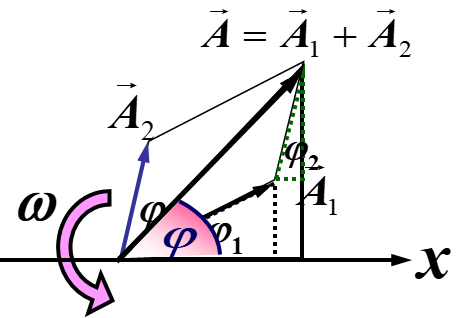
\includegraphics[width=2.45694in,height=1.70208in]{./media/media/image2.png}

图2 旋转矢量法合成同频率同方向的光

\hypertarget{ux5149ux5f3aux7684ux8868ux793a}{%
\subsubsection{光强的表示}\label{ux5149ux5f3aux7684ux8868ux793a}}

本文围绕光的干涉现象,阐述其波动叠加本质与基本规律,深入剖析相干条件的核心要素,并推导相干与非相干叠加场景下的光强计算方法及物理意义。

\textbf{光矢量与光强}

光矢量 \(\overrightarrow{E}\) :光是电磁波,电场强度矢量 \(\overrightarrow{E}\) 是光的振动矢量,称为光矢量,它的振动是光现象的主要体现。

光强 \(I\) :光的强度(光强)与光矢量振幅 \(E_{0}\) 的平方成正比,即 \(I \propto E_{0}^{2}\) ,光强越大,干涉光越亮。

\begin{quote}
\textbf{光的独立性与叠加原理}
\end{quote}

光的独立性原理:两列光在空间相遇时,各自的传播规律不受对方影响,继续保持原来的传播特性(如频率、波长、振动方向等)。\\
光的叠加原理:两列或多列光在空间某点相遇时,该点的光矢量是各列光在该点光矢量的矢量和。

\textbf{相干条件}

两束光的相干叠加(产生稳定干涉条纹)需满足以下条件:

\begin{enumerate}
\def\labelenumi{\arabic{enumi}.}
\item
  频率相同:\(\omega_{1} = \omega_{2}\)( \(\omega\) 为角频率,频率 \(\nu = \frac{\omega}{2\pi}\) ,频率相同意味着振动的"快慢"一致)。

  2.振动方向夹角稳定且非垂直:两列光的振动方向(光矢量方向)的夹角 \(\alpha\) 不随时间 \(t\) 变化,且 \(\alpha \neq \frac{\pi}{2}\)(若垂直,光矢量叠加时部分分量会抵消,难以形成稳定干涉)。
\end{enumerate}

3.相位差稳定:两列光的相位差 \(\Delta\varphi\) 不随着时间 \(t\) 变化(相位差稳定才能保证叠加后光强的分布趋于稳定)。

\textbf{光强的叠加}

相干叠加:若两列光满足相干条件,叠加后的光强为 \(I = I_{1} + I_{2} + 2\sqrt{I_{1}I_{2}}cos\Delta\varphi_{0}\) 。其中, \(2\sqrt{I_{1}I_{2}}cos\Delta\varphi\) 是干涉项,它使光强分布随相位差 \(\Delta\varphi\) 变化:

当 \(\Delta\varphi = \pm 2\text{kπ}\text{\ }(k = 0,1,2,\ldots)\) 时, \(cos\Delta\varphi = 1\) ,光强 \(I = I_{1} + I_{2} + 2\sqrt{I_{1}I_{2}} = \left( \sqrt{I_{1}} + \sqrt{I_{2}} \right)^{2}\) ,达到相长干涉(光强最大)。

当 \(\Delta\varphi = \pm (2k - 1)\pi(k = 1,2,\ldots)\) 时, \(cos\Delta\varphi = - 1\) ,光强 \(I = I_{1} + I_{2} - 2\sqrt{I_{1}I_{2}} = \left( \sqrt{I_{1}} - \sqrt{I_{2}} \right)^{2}\) ,达到相消干涉(光强最小,若 \(I_{1} = I_{2}\) ,则光强为 0 )。

\hypertarget{ux5149ux7a0bux548cux5149ux5dee}{%
\subsubsection{光程和光差}\label{ux5149ux7a0bux548cux5149ux5dee}}

设某一频率为 f的单色光在真空中的传播速度为 c,波长为 λ。当该光在折射率为 n 的介质中传播时,其速度变为 v,波长变为 ′λ′。

\[\lambda_{n} = \frac{u}{v} = \frac{c/n}{v} = \frac{\lambda}{n}\]

上述公式表明,特定频率的光在折射率为 n 的介质中传播时,其波长为真空中的波长的 1/n\hspace{0pt} 倍。根据波动理论,当每束光从光源传播至相遇点经过 1 个单位距离后,其相位变化量为

\[\Delta\phi = 2\pi\frac{l}{\lambda}\]

由于同一频率的光在不同介质中的波长各不相同,因此上述公式中的 λ′′ 应该理解为光在相应介质中的波长。因此,当单色光在折射率为 n的介质中传播一定距离后,其相位变化量为

\[\Delta\phi = 2\pi\frac{l}{\lambda_{n}} = 2\pi\frac{\text{nl}}{\lambda}\]

上述公式表明,光在折射率为 n的介质中传播一定距离 d后,其相位变化量与光在真空中传播相同距离时的相位变化量是相等的。因此,我们将光在介质中传播的距离 d与该介质的折射率 n的乘积 n⋅d 称为光程。

\textbf{光程差与干涉的关系}

如图 3 所示,若两个初相均为 \(\phi\) 的相干光源 \(S_{1},\text{\ }S_{2}\) 发出的光在 P 点相遇,则它们在 P 点的相位差为

\[\Delta\phi = \left( \phi - 2\pi\frac{n_{2}r_{2}}{\lambda} \right) - \left( \phi - 2\pi\frac{n_{1}r_{1}}{\lambda} \right) = \frac{2\pi}{\lambda}\left( n_{1}r_{1} - n_{2}r_{2} \right)\]

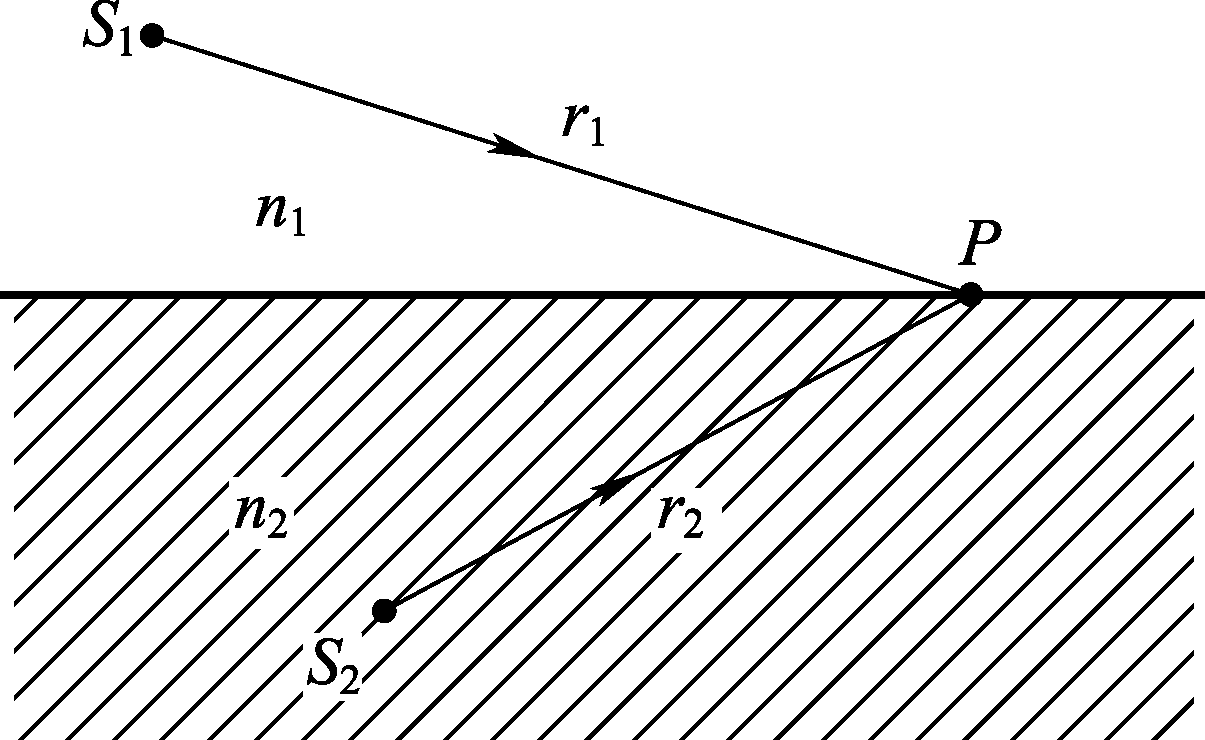
\includegraphics[width=1.97361in,height=1.23264in]{./media/media/image3.png}

图3 计算相干光的光程差

令 \(n_{1}r_{1} - n_{2}r_{2} = \delta,\delta\) 称为两束光的光程差,其中\(n_{1}\)和\(n_{2}\)是两种介质的折射率,则上式可写为

\[\Delta\phi = \frac{2\text{πδ}}{\lambda}\]

因此,在波动光学中,干涉相长和干涉相消的条件可以通过光程差来进行表述

\[\delta = \pm \text{kλ}(k = 0,1,2,\cdots)\text{~}\text{干涉相长}\text{\ (}\text{明纹}\text{)}\]

\[\delta = \pm (2k + 1)\lambda/2(k = 0,1,2,\cdots)\text{~}\text{干涉相消}\text{\ (}\text{暗纹}\text{)}\]

\end{document}
